\documentclass[12pt,a4paper]{article}
\usepackage[utf8]{vietnam}
\usepackage{amsmath}
\usepackage{amsfonts}
\usepackage{amssymb}
\usepackage{graphicx}
\usepackage{float}
\usepackage{tablefootnote}
\usepackage{adjustbox}
\usepackage{multirow}
\usepackage[left=2cm,right=2cm,top=2cm,bottom=2cm]{geometry}
\author{Nguyễn Văn Lộc - 20120131}
\title{\textbf{A Tutorial on Dynamic Programming}}
\begin{document}
\maketitle
\section{Ví dụ 1}
Chúng ta sẽ bắt đầu bằng một bài toán về ngân sách dự trù cho nguồn vốn. Một tập đoàn có \(5\) triệu dollar, phân phối tới \(3\) chi nhánh, cho những hoạt động mở rộng. Mỗi chi nhánh đã nộp một vài bản kế hoạch về việc họ sẽ sử dụng số tiền như thế nào. Mỗi kế hoạch cung cấp chi phí mở rộng (\(c\)) và tổng doanh thu dự kiến (\(r\)). Bảng sau cung cấp thông tin chi tiết về các kế hoạch (trong đó \(c_i\) và \(r_i\) là thông số của chi nhánh thứ \(i\)):\\
\begin{table}[h]
\begin{center}
\begin{tabular}{|c|c|c|c|c|c|c|}
\hline 
Kế hoạch & \(c_1\) & \(r_1\) & \(c_2\) & \(r_2\) & \(c_3\) & \(r_3\) \\ 
\hline 
1 & \(0\) & \(0\) & \(0\) & \(0\) & \(0\) & \(0\) \\ 
\hline 
2 & \(1\) & \(5\) & \(2\) & \(8\) & \(1\) & \(4\) \\ 
\hline 
3 & \(2\) & \(6\)  & \(3\) & \(9\) & - & - \\ 
\hline 
4 & - & - & \(4\) & \(12\) & - & - \\ 
\hline 
\end{tabular} 
\caption{Các khả năng đầu tư}
\end{center}
\end{table}
Mỗi chi nhánh chỉ được phép thực hiện một trong số những kế hoạch của họ. Mục tiêu là tối đa hóa lợi nhuận mà tập đoàn thu được từ \(5\) triệu dollar ban đầu. Giả sử rằng phần tiền không được sử dụng trong \(5\) triệu dollar này sẽ bị mất (có thể xem xét bài toán về việc một giả thiết hợp lí hơn sẽ ảnh hưởng như thế nào đến bài toán như là một bài tập).
Một cách tiếp cận trực tiếp cho bài toán này là thử tất cả các trường hợp và chọn ra trường hợp tốt nhất. Trong trường hợp này, ta chỉ có \(3 \times 4 \times 2 = 24\) cách để phân phối nguồn tiền. Có nhiều cách trong số đó không thể thực hiện (ví dụ, kế hoạch 3, 4 và 1 cho ba chi nhánh tốn \(6\) triệu dollar). Những trường hợp khác có thể đạt được, nhưng rất kém triển vọng (ví dụ, kế hoạch 1, 1 và 2 chỉ mang về \(4\) triệu dollar).\\
Những khuyết điểm của cách làm liệt kê toàn bộ bao gồm:
\begin{itemize}
\item Với những bài toán lớn hơn, cách liệt kê toàn bộ có thể không thực hiện được.
\item Những tổ hợp không khả thi không thể được coi là hiển nhiên đúng, dẫn đến kém hiệu quả.
\item Thông tin về những trường hợp đã được khảo sát trước đó không được sử dụng để dự đoán trường hợp "kém", hoặc trường hợp không xảy ra.
\end{itemize}
Lưu ý rằng bài toán này không thể được xây dựng thành một chương trình tuyến tính (linear program), vì doanh thu nhận được không phải một hàm tuyến tính.\\
Một cách để tìm lời giải cho bài toán như sau:
Ta sẽ chia bài toán thành 3 giai đoạn (stage): mỗi giai đoạn đại diện cho số tiền được phân phối tới từng chi nhánh. Vì vậy, giai đoạn 1 thể hiện cho số tiền được phân phối cho chi nhánh 1, giai đoạn 2 là số tiền cho chi nhánh 2 và giai đoạn 3 cho chi nhánh 3. Ta sẽ tự đặt ra thứ tự cho 3 giai đoạn, trước hết ta sẽ cung cấp tiền đến chi nhánh 1, sau đó đến chi nhánh 2 rồi chi nhánh 3.\\
Mỗi giai đoạn được chia thành các trạng thái. Mỗi trạng thái chứa đựng thông tin cần thiết để đi từ một giai đoạn tới giai đoạn tiếp theo. Trong trường hợp này, những trạng thái cho giai đoạn 1, 2, 3 là
\begin{itemize}
\item \(\left\{ {0,1,2,3,4,5} \right\}:\) lượng tiền sử dụng cho chi nhánh 1, kí hiệu là \(x_1,\)
\item \(\left\{ {0,1,2,3,4,5} \right\}:\) lượng tiền sử dụng ở cho nhánh 1 và 2, kí hiệu là \(x_2,\) và
\item \(\left\{ {5} \right\}:\) lượng tiền sử dụng ở cả 3 chi nhánh, kí hiệu là \(x_3.\)
\end{itemize}
Không giống như quy hoạch tuyến tính, \(x_i\) không đại diện cho lượng biến đổi quyết định (decision variables), mà chỉ là sự thể hiện đơn giản cho một trạng thái chung trong giai đoạn.\\
Liên kết với mỗi trạng thái là một doanh thu. Lưu ý rằng để quyết định ở giai đoạn 3, ta chỉ cần biết lượng tiền đã sử dụng ở giai đoạn 1 và 2, không cần biết chúng được sử dụng như thế nào. Một lưu ý khác là ta đang muốn \(x_3\) nhận giá trị là \(5.\)
Ta sẽ cố gắng tìm ra lợi nhuận gắn với mỗi trạng thái. Một khả năng dễ thấy là trong giai đoạn \(1,\) trạng thái là \(x_1.\) Bảng \ref{bang2} sẽ cho ta các khả năng của \(x_1.\)\\
\begin{table}[H]
\begin{center}
\label{bang2}
\begin{tabular}{|c|c|c|}
\hline 
Nguồn vốn sẵn có \(x_1\) & Kế hoạch khả quan & Doanh thu \\ 
\hline 
0 & 1 & 0 \\ 
\hline 
1 & 2 & 5 \\ 
\hline 
2 & 3 & 6 \\ 
\hline 
3 & 3 & 6 \\ 
\hline 
4 & 3 & 6 \\ 
\hline 
5 & 3 & 6 \\ 
\hline 
\end{tabular} 
\caption{Số liệu ở giai đoạn 1}
\end{center}
\end{table}
Bây giờ ta đã sẵn sàng để xử lí tính toán cho giai đoạn 2. Trong trường hợp này, ta muốn tìm ra lời giải tốt nhất cho cả giai đoạn 1 và 2. Nếu ta muốn tính toán doanh thu tối đa từ \(x_2\) cho trước, ta chỉ cần xét tất cả các kế hoạch của chi nhánh 2, phân phối một nguồn vốn sẵn có cho chi nhánh 2, và sử dụng bảng trên để xem xét chi nhánh 1 sẽ sử dụng phần còn lại như thế nào.\\
Ví dụ, giả sử ta muốn định rõ sự phân phối cho trạng thái \(x_2 = 4.\) Trong giai đoạn 2, ta có thể làm một trong các kế hoạch sau:
\begin{itemize}
\item Kế hoạch 1 cho doanh thu \(0,\) để lại \(4\) cho giai đoạn \(1,\) thu được doanh thu \(6.\) Tổng doanh thu: \(6.\)
\item Kế hoạch 2 cho doanh thu \(8,\) để lại \(2\) cho giai đoạn \(1,\) thu được doanh thu \(6.\) Tổng doanh thu: \(14.\)
\item Kế hoạch 3 cho doanh thu \(9,\) để lại \(1\) cho giai đoạn \(1,\) thu được doanh thu \(5.\) Tổng doanh thu: \(14.\)
\item Kế hoạch 4 cho doanh thu \(12,\) để lại \(0\) cho giai đoạn \(1,\) thu được doanh thu \(0.\) Tổng doanh thu: \(12.\)
\end{itemize}
Vậy, giải pháp tốt nhất với \(x_2 = 4\) là kế hoạch 2 cho chi nhánh 1 và kế hoạch 3 cho chi nhánh 2, hoặc kế hoạch 3 cho chi nhánh 1 và kế hoạch 2 cho chi nhánh 2, cả hai trường hợp đều cho tổng doanh thu là \(14.\) Phần còn lại của bảng 3 được điền tương tự.\\
\begin{table}[H]
\begin{center}
\label{bang3}
\begin{tabular}{|c|c|c|}
\hline 
Nguồn vốn sẵn có \(x_2\) & Kế hoạch khả quan & Tổng lợi nhuận giai đoạn 1 và giai đoạn 2 \\ 
\hline 
0 & 1 & 0 \\ 
\hline 
1 & 1 & 5 \\ 
\hline 
2 & 2 & 8 \\ 
\hline 
3 & 2 & 13 \\ 
\hline 
4 & 2 hoặc 3 & 14 \\ 
\hline 
5 & 4 & 17 \\ 
\hline 
\end{tabular} 
\end{center}
\caption{Số liệu ở giai đoạn 2}
\end{table}
Ta xét đến giai đoạn 3. Giá trị duy nhất mà ta mong muốn là \(x_3 = 5.\) Một lần nữa, ta xét tất cả kế hoạch ở giai đoạn này, xác định số lượng tiền còn lại và sử dụng bảng 3 để quyết định giá trị cho các giai đoạn trước. Vì vậy, ta có thể xét các trường hợp sau đây ở giai đoạn 3:
\begin{itemize}
\item Kế hoạch 1 cho doanh thu \(0\), còn lại \(5.\) Các giai đoạn trước cho doanh thu \(17.\) Tổng doanh thu: \(17.\)
\item Kế hoạch 1 cho doanh thu \(4\), còn lại \(4.\) Các giai đoạn trước cho doanh thu \(14.\) Tổng doanh thu: \(18.\)
\end{itemize}
Vì vậy, giải pháp tối ưu là áp dụng kế hoạch 2 ở chi nhánh 3, kế hoạch 2 hoặc 3 ở chi nhánh 2, và kế hoạch 3 hoặc 2 (theo thứ tự) ở chi nhánh 1. Tổng doanh thu là \(18.\)\\
Từ quá trình này, ta có thể nhận thấy việc xử lí tính toán được tiến hành bằng \textit{đệ quy}. Tính toán ở giai đoạn 2 dựa trên giai đoạn 1, giai đoạn 3 dựa trên giai đoạn 2. Thật vậy, giả sử ta đang ở một trạng thái, tất cả quyết định trong tương lai được đưa ra một cách độc lập với việc ta đi vào trạng thái đó như thế nào. Đây là \textit{nguyên lí tối ưu} (principle of optimality) và toàn bộ vấn đề quy hoạch động đều dựa trên giả thiết này.\\
Ta có thể tổng hợp những tính toán này thành công thức sau đây:
\begin{center}
Kí hiệu \(r\left( {{k_j}} \right)\) là doanh thu của kế hoạch \({k_j}\) ở giai đoạn \(j,\) và \(c\left( {{k_j}} \right)\) là chi phí tương ứng. Đặt \({f_j}\left( {{x_j}} \right)\) là doanh thu của trạng thái \({x_j}\) ở giai đoạn \(j.\) Khi đó, ta được
\[{f_1}\left( {{x_1}} \right) = \mathop {\max }\limits_{{k_1}:c\left( {{k_1}} \right) \leqslant {x_1}} \left\{ {r\left( {{k_1}} \right)} \right\}\]
và 
\[{f_j}\left( {{x_j}} \right) = \mathop {\max }\limits_{{k_j}:c\left( {{k_j}} \right) \leqslant {x_j}} \left\{ {r\left( {{k_j}} \right) + {f_{j - 1}}\left( {{x_j} - c\left( {{k_j}} \right)} \right)} \right\},j = 2,3.\]
\end{center}
Những tính toán ở phía bên trên mà ta đã thực hiện là để xác định những hám số này.\\
Ta đã xử lí theo một quy trình tiến tới (forward procedure). Ngoài ra, ta vẫn có thể tính toán từ giai đoạn "cuối cùng" ngược trở về giai đoạn đàu tiên. Ta có thể định nghĩa
\begin{itemize}
\item \({y_1} = \) lượng tiền sử dụng ở giai đoạn 1, 2 và 3,
\item \({y_2} = \) lượng tiền sử dụng ở giai đoạn 2 và 3, và
\item \({y_3} = \) lượng tiền sử dụng ở giai đoạn 3.
\end{itemize}
Quá trình này được gọi là \textit{đệ quy quay lui} (backward recursion), được biểu diễn bằng đồ thị trong hình \ref{hinh1}.
\begin{center}
\begin{figure}[H]
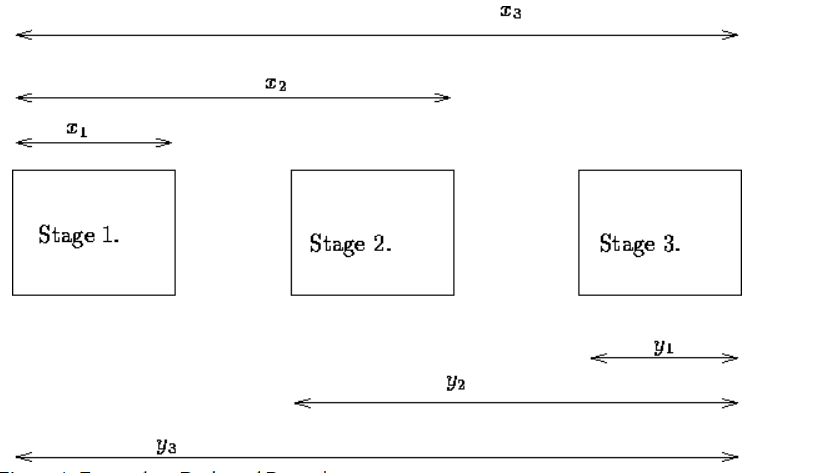
\includegraphics[scale=1]{hinh1}
\caption{Đệ quy tiến tới và đệ quy quay lui (forward vs backward recursion)}
\label{hinh1}
\end{figure}
\end{center}
Các công thức tương ứng là
\begin{itemize}
\item \({f_3}\left( {{y_3}} \right)\) là doanh thu tối ưu ở giai đoạn 3 với \(y_3\) cho trước,
\item \({f_2}\left( {{y_2}} \right)\) là doanh thu tối ưu ở giai đoạn 2 và 3 với \(y_2\) cho trước, và
\item \({f_1}\left( {{y_1}} \right)\) là doanh thu tối ưu ở giai đoạn 1, 2 và 3 với \(y_1\) cho trước.
\end{itemize}
Các công thức đệ quy là
\[{f_3}\left( {{y_3}} \right) = \mathop {\max }\limits_{{k_3}:c\left( {{k_3}} \right) \leqslant {y_3}} \left\{ {r\left( {{k_3}} \right)} \right\}\]
và \[{f_j}\left( {{x_j}} \right) = \mathop {\max }\limits_{{k_j}:c\left( {{k_j}} \right) \leqslant {y_j}} \left\{ {r\left( {{k_j}} \right) + {f_{j + 1}}\left( {{y_j} - c\left( {{k_j}} \right)} \right)} \right\}.\]
Nếu ta tính toán như thế này, ta sẽ thu được kết quả giống như phương pháp đệ quy tiến tới.\\
Chắc bạn sẽ thắc mắc tại sao tôi lại giới thiệu đệ quy quay lui, rõ ràng là đệ quy tiến tới trông có vẻ tự nhiên hơn. Trong trường hợp cụ thể này, thứ tự các bước không tạo ra sự khác biệt nào. Mặc dù vậy, trong nhiều trường hợp khác, có thể một phương pháp sẽ có nhiều lợi ích hơn phương pháp còn lại. Nói chung là phương pháp đệ quy quay lui được phát minh để trở nên hiệu quả hơn trong nhiều ứng dụng. Vì vậy, trong tương lai, tôi sẽ chỉ trình bày phương pháp đệ quy quay lui, trừ trường hợp tôi muốn so sánh sự tương phản của hai phương pháp.
\section{Ví dụ 2}
Quy hoạch động đôi khi trông rất quen thuộc. Cả thuật toán tìm đường đi ngắn nhất và phương pháp cho CPM project scheduling đều có nhiều điểm chung với nó.
Ta sẽ xem xét một bài toán tìm đường đi ngắn nhất cụ thể. Giả sử ta cần đi từ \(A\) đến \(J\) trong một mạng lưới đường phố như hình \ref{hinh2}.
\begin{center}
\begin{figure}[H]
\label{hinh2}
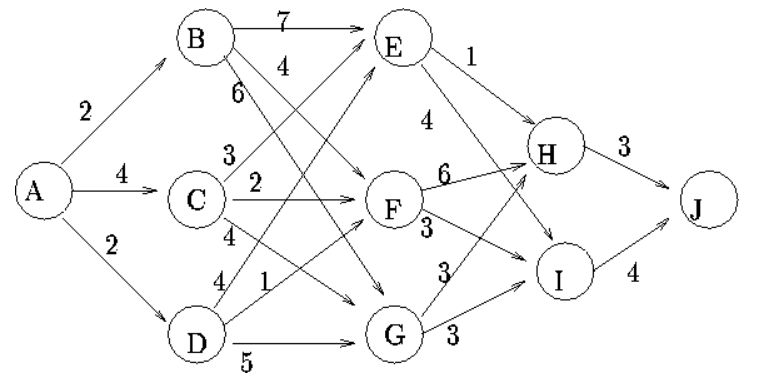
\includegraphics[scale=1]{hinh2}
\caption{Mạng lưới đường phố}
\end{figure}
\end{center}
Con số trên mỗi cung thể hiện khoảng cách giữa hai điểm. Do cấu trúc đặc biệt của bài toán này, ta có thể chia nó thành từng giai đoạn. Giai đoạn 1 chứa đỉnh \(A\), giai đoạn 2 chứa đỉnh \(B, C\) và \(D,\) giai đoạn 3 chứa đỉnh \(E, F\) và \(G,\) giai đoạn 4 chứa đỉnh \(H\) và \(I,\) và giai đoạn 5 chứa đỉnh \(J.\) Mỗi trạng thái trong từng giai đoạn tương ứng với tên của các đỉnh. Vì vậy, giai đoạn 3 chứa các trạng thái \(E, F\) và \(G.\)\\
Nếu ta kí hiệu \(S\) là một đỉnh trong giai đoạn \(j\) và đặt \({f_j}\left( S \right)\) là khoảng cách ngắn nhất từ đỉnh \(S\) tới điểm đến \(J,\) ta có thể viết
\[{f_j}\left( S \right) = \mathop {\min }\limits_{nodes\_Z\_in\_stage\_j + 1} \left\{ {{c_{SZ}} + {f_{j + 1}}\left( Z \right)} \right\}\]
với \({c_{SZ}}\) là độ dài của cung \(SZ.\) Đây là công thức đệ quy cần dùng để giải bài toán này. Ta bắt đầu với việc đặt \({f_5}\left( J \right) = 0.\) Phần còn lại của bài toán được xử lí như sau:\\
\textbf{\textit{Giai đoạn 4.}}\\
Trong giai đoạn 4, không có quyết định nào thực sự được đưa ra, vì ta cần phải đi đến điểm \(J.\) Vì vậy, ta thu được:
\begin{itemize}
\item \({f_4}\left( H \right) = 3\) khi đi tới \(J.\)
\item \({f_4}\left( J \right) = 4\) khi đi tới \(J.\)
\end{itemize}
\textbf{\textit{Giai đoạn 3.}}\\
Ở giai đoạn này thì ta có nhiều sự lựa chọn hơn. Sau đây là cách mà ta tính \({f_3}\left( F \right).\) Từ \(F\) ta có thể đi đến \(H\) hoặc \(I.\) Chi phí để đi đến \(H\) là \(6,\) sau đó ta cần tốn \({f_4}\left( H \right) = 3.\) Tổng chi phí là \(9.\) Chi phí để đi đến \(I\) là \(3,\) sau đó ta cần tốn \({f_4}\left( J \right) = 4.\) Tổng chi phí là \(7.\) Vì vậy, nếu ta đang ở \(F,\) tốt nhất là đi đến \(I.\) Tổng chi phí là \(7,\) vậy \({f_3}\left( F \right) = 7.\)\\
Bảng sau cho ta tất cả số liệu ở giai đoạn 3:
\begin{center}
\begin{table}[H]
\begin{tabular}{|c|c|c|c|c|}
\hline 
\(S_3\) & \multicolumn{2}{c|}{\({c_{{S_3}{Z_3}}} + {f_4}\left( {{Z_3}} \right)\)} & \({f_3}\left( {{S_3}} \right)\) & Quyết định đi đến \\ 
\hline 
• & \(H\) & \(I\) & • & • \\ 
\hline 
\(E\) & \(4\) & \(8\) & \(4\) & \(H\) \\ 
\hline 
\(F\) & \(9\)  & \(7\) & \(7\)  & \(I\) \\ 
\hline 
\(G\) & \(6\) & \(7\) & \(6\) & \(H\) \\ 
\hline 
\end{tabular}
\end{table}
\end{center} 
Ta có thể tiếp tục tính toán từng giai đoạn, kết thúc tính toán ở một giai đoạn trước khi đến với giai đoạn ngay trước nó. Kết quả là:\\
\textbf{\textit{Giai đoạn 2.}}
\begin{center}
\begin{table}[H]
\begin{tabular}{|c|c|c|c|c|c|}
\hline 
\(S_2\) & \multicolumn{3}{c|}{\({c_{{S_2}{Z_2}}} + {f_3}\left( {{Z_2}} \right)\)} & \({f_2}\left( {{S_2}} \right)\) & Quyết định đi đến \\ 
\hline 
• & \(E\) & \(F\) & \(G\) & • & • \\ 
\hline 
\(B\) & \(11\) & \(11\) & \(12\) & \(11\) & \(E\) hoặc \(F\) \\ 
\hline 
\(C\) & \(7\) & \(9\) & \(10\) & \(7\) & \(E\) \\ 
\hline 
\(D\) & \(8\) & \(8\) & \(11\) & \(8\) & \(E\) hoặc \(F\) \\ 
\hline 
\end{tabular}
\end{table}
\end{center} 
\textbf{\textit{Giai đoạn 1.}}
\begin{center}
\begin{table}[H]
\begin{tabular}{|c|c|c|c|c|c|}
\hline 
\(S_1\) & \multicolumn{3}{c|}{\({c_{{S_1}{Z_1}}} + {f_2}\left( {{Z_1}} \right)\)} & \({f_1}\left( {{S_1}} \right)\) & Quyết định đi đến \\ 
\hline 
• & \(B\) & \(C\) & \(D\) & • & • \\ 
\hline 
\(A\) & \(13\) & \(11\) & \(11\) & \(11\) & \(C\) hoặc \(D\) \\ 
\hline 
\end{tabular} 
\end{table}
\end{center}
\section{Những đặc tính chung}
Ta có thể rút ra một vài đặc tính chung của hai ví dụ vừa qua và cho cả quy hoạch động, đó là:
\begin{itemize}
\item Bài toán có thể được chia thành nhiều \textit{giai đoạn} và một \textit{quyết định} cần phải được đưa ra ở mỗi giai đoạn.
\item Mỗi giai đoạn có một số lượng \textit{trạng thái} liên kết với nó.
\item Quyết định tại mỗi giai đoạn biến đổi một trạng thái thành một trạng thái ở giai đoạn kế tiếp.\\
Trạng thái ở bài toán ngân sách dự trù cho nguồn vốn là số lượng tiền sử dụng ở mỗi điểm. Trạng thái ở bài toán tìm đường đi ngắn nhất là một đỉnh.
\item Giả sử ta ở một trạng thái cho trước, quyết định tối ưu cho từng trạng thái trong những trạng thái còn lại không phụ thuộc vào trạng thái hoặc quyết định trước đó.\\
Trong bài toán nguồn vốn, ta không cần biết nguồn tiền được sử dụng như thế nào ở giai đoạn trước đó, chỉ cần biết đã dùng bao nhiêu. Trong bài toán đường đi ngắn nhất, ta không cần biết đã đi đến đỉnh đó như thế nào.
\item Tồn tại một mối liên hệ đệ quy xác định quyết định tối ưu cho giai đoạn \(j,\) biết rằng giai đoạn \(j + 1\) đã được giải quyết.
\item Giai đoạn cuối cùng phải tự giải quyết.
\end{itemize}
Hai tính chất cuối cùng đã được hợp nhất trong công thức đệ quy đã cho phía trên.\\
Một kĩ năng cần thiết trong quy hoạch động, và trong các bài toán có chứa quy hoạch động, là tách bài toán thành các giai đoạn và các trạng thái tương ứng với từng giai đoạn. Nếu ta có thể làm được điều này thì từ công thức đệ quy có thể tìm ra cá giá trị môt cách dễ dàng. Vì sự khó khăn khi xác định các giai đoạn và trạng thái, ta sẽ thử làm một vài ví dụ.
\section{Bài toán xếp ba lô (Knapsack problem)}
Bài toán xếp ba lô là một bài toán điển hình khi làm việc với số nguyên với một constraint. Mỗi vật phẩm trong bài toán xếp ba lô có một kích thước (size) và một phúc lợi (benefit). Sức chứa của ba lô được định rõ. Ta cần phải xếp đồ vào ba lô như thế nào để tối đa hóa phúc lợi nhận được? Lấy ví dụ, giả sử ta có ba vật phẩm như trong bảng \ref{bang4} và giả sử sức chứa của ba lô là \(5.\)
\begin{center}
\begin{table}[H]
\label{bang4}
\begin{tabular}{|c|c|c|}
\hline 
Vật phẩm \(\left( {j} \right)\) & Khối lượng \(\left( {w_j} \right)\) & Phúc lợi \(\left( {b_j} \right)\) \\ 
\hline 
1 & 2 & 65 \\ 
\hline 
2 & 3 & 80 \\ 
\hline 
3 & 1 & 30 \\ 
\hline 
\end{tabular} 
\caption{Các vật phẩm trong ba lô}
\end{table}
\end{center}
Các giai đoạn đại diện cho các vật phẩm: ta có ba giai đoạn \(j = 1, 2, 3.\) Trạng thái \(y_j\) ở giai đoạn \(j\) là tổng khối lượng của các vật phẩm \(j\) và những vật phẩm trong ba lô. Quyết định ở giai đoạn \(j\) là bỏ bao nhiêu vật phẩm \(j\) vào trong ba lô. Ta đặt giá trị này là \(k_j.\)\\
Công thức đệ quy được dẫn tới như sau. Ta đặt \({f_j}\left( {{y_j}} \right)\) là giá trị phúc lợi nhận được khi sử dụng \(y_j\) đơn vị không gian của ba lô để chứ vật phẩm \(j.\) Đặt \(\left\lfloor a \right\rfloor \) là số nguyên lớn nhất không vượt quá \(a.\)
\begin{itemize}
\item \({f_3}\left( {{y_j}} \right) = 30{y_j}\)
\item \({f_j}\left( {{y_j}} \right) = \mathop {\max }\limits_{{k_j} \leqslant \left\lfloor {\frac{{{y_j}}}{{{w_j}}}} \right\rfloor } \left\{ {{b_j}{k_j} + {f_{j + 1}}\left( {{y_j} - {w_j}{k_j}} \right)} \right\}.\)
\end{itemize}
\section{Một công thức thay thế}
Ta còn một công thức khác cho bài toán xếp ba lô. Điều này thể hiện tính bất kì trong định nghĩa của chúng ta về giai đoạn, trạng thái và quyết định. Ngoài ra, nó còn nói lên sự linh hoạt trong các quy tắc về quy hoạch động. Định nghĩa của ta đòi hỏi một quyết định ở mỗi giai đoạn trước khi sang giai đoạn kế tiếp (mà ta đã tính dựa vào đệ quy quay lui). Thật ra, ta có thể đến bất kì giai đoạn nào mà ta đã tính toán trước đó. Điều này có thể giúp ta linh hoạt hơn trong việc xử lí tính toán.\\
Tôi đang muốn trình bày đệ quy tiến tới. Với một bài toán xếp ba lô, ta sẽ đánh số cho một giai đoạn là \(w.\) Chỉ có một trạng thái mỗi giai đoạn. Đặt \(g\left( w \right)\) là số lượng phúc lợi tối đa mà ta nhận được khi sử dụng \(w\) đơn vị không gian trong ba lô. Tiếp tục sử dụng \(w_j\) và \(b_j\) là khối lượng và phúc lợi, theo thứ tự, của vật phẩm \(j,\) công thức sau đây thể hiện mối tương quan giữa \(g\left( w \right)\) và các giá trị \(g\) đã được tính toán trước đó:
\[g\left( w \right) = \mathop {\max }\limits_j \left\{ {{b_j} + g\left( {w - {w_j}} \right)} \right\}\]
Từ trực giác, ta nhận thấy rằng, để làm đầy \(w\) đơn vị không gian của ba lô, ta cần phải kết thúc bằng thao tác thêm một vài vật phẩm. Nếu ta thêm vật phẩm \(j,\) ta cần phải kết thúc với một ba lô có \(w - w_j\) đơn vị không gian. Để diễn tả công thức trên, ta có
\begin{itemize}
\item \(g\left( 0 \right) = 0,\)
\item \(g\left( 1 \right) = 30,\) thêm vật phẩm 3,
\item \(g\left( 2 \right) = \max \left\{ {65 + g\left( 0 \right) = 65,30 + g\left( 1 \right) = 60} \right\} = 65,\) thêm vật phẩm 1,
\item \(g\left( 3 \right) = \max \left\{ {65 + g\left( 1 \right) = 95,80 + g\left( 0 \right) = 80,30 + g\left( 2 \right) = 95} \right\} = 95,\) thêm vật phẩm 1 hoặc 3,
\item \(g\left( 4 \right) = \max \left\{ {65 + g\left( 2 \right) = 130,80 + g\left( 1 \right) = 110,30 + g\left( 3 \right) = 125} \right\} = 130,\) thêm vật phẩm 1,
\item \(g\left( 5 \right) = \max \left\{ {65 + g\left( 3 \right) = 160,80 + g\left( 2 \right) = 145,30 + g\left( 4 \right) = 160} \right\} = 160,\) thêm vật phẩm 1 hoặc 3.
\end{itemize}
Tổng phúc lợi tối đa thu được là \(160,\) bằng cách thêm \(2\) vật phẩm 1 và \(1\) vật phẩm 3.
\section{Thay thế trang thiết bị}
Trong bài tập về network, ta đã thấy cách tạo ra công thức và giải quyết một bài toán thay thế thiết bị bằng thuật toán tìm đường đi ngắn nhất. Bây giờ ta sẽ tìm một công thức thay thế bằng quy hoạch động.\\
Giả sử một cửa hàng cần một cỗ máy trong khoảng thời gian \(5\) năm tới. Một chiếc máy mới có giá \(1000\) dollar. Chi phí bảo trì máy trong năm thứ \(i\) từ lúc vận hành là \(m_1 = 60, m_2 = 80\) và \(m_3 = 120\) dollar. Một chiếc máy có thể được giữ trong vòng \(3\) năm trước khi đem ra giao dịch. Giá trị giao dịch sau \(i\) năm là \(s_1 = 800, s_2 = 600\) và \(s_3 = 500\) dollar. Cửa hàng đó phải làm thế nào để tối thiểu hóa chi phí trong khoảng thời gian \(5\) năm?\\
Ta sẽ xem mỗi giai đoạn tương ứng với một năm. Trạng thái trong một giai đoạn là tuổi của cỗ máy trong năm đó. Quyết định là giữ hoặc trao đổi để lấy một chiếc máy mới. Đặt \({f_t}\left( x \right)\) là chi phí nhỏ nhất phát sinh trong khoảng thời gian từ năm thứ \(t\) đến năm thứ \(5,\) biết rằng cỗ máy được \(x\) tuổi vào năm thứ \(t.\)\\
Do ta bắt buộc phải đem ra giao dịch tại năm thứ \(5,\) 
\[{f_5}\left( x \right) =  - {s_x}.\]
Bây giờ ta sẽ xét các khoảng thời gian khác. Nếu ta có một cỗ máy được \(3\) tuổi vào năm thứ \(t,\) ta sẽ phải mang ra giao dịch, vì vậy
\[{f_t}\left( 3 \right) =  - 500 + 1000 + 60 + {f_{t + 1}}\left( 1 \right)\left( {Trade} \right)\]
Nếu ta có một cỗ máy \(2\) tuổi, ta có thể mang ra giao dịch hoặc giữ lại
\begin{itemize}
\item Giao dịch tốn \( - 600 + 1000 + 60 + {f_{t + 1}}\left( 1 \right),\)
\item Giữ lại tốn \(120 + {f_{t + 1}}\left( 3 \right).\)
\end{itemize}
Vì vậy, việc tốt nhất ta cần làm là giá trị nhỏ nhất của hai giá trị này.\\
Tương tự
\[{f_t}\left( 1 \right) = \min \left\{ { - 800 + 1000 + 60 + {f_{t + 1}}\left( 1 \right),80 + {f_{t + 1}}\left( 2 \right)} \right\}.\]
Cuối cùng, tại năm thứ \(0,\) ta cần phải mua, vì vậy
\[{f_0}\left( 0 \right) = 1000 + 60 + {f_1}\left( 1 \right).\]
Bài toán có thể được giải quyết bằng đệ quy quay lui như sau:\\
\textbf{\textit{Giai đoạn 5.}}
\begin{center}
\begin{table}[H]
\begin{tabular}{|c|c|}
\hline 
Tuổi \(x\) & \(f_5 \left( x \right)\) \\ 
\hline 
\(1\) & \(-800\) \\ 
\hline 
\(2\) & \(-600\) \\ 
\hline 
\(3\) & \(-500\) \\ 
\hline 
\end{tabular} 
\end{table}
\end{center}
\textbf{\textit{Giai đoạn 4.}}
\begin{center}
\begin{table}[H]
\begin{tabular}{|c|c|c|c|c|}
\hline 
Tuổi \(x\) & Giao dịch & Giữ lại & \(f_4 \left( x \right)\) & Quyết định \\ 
\hline 
\(1\) & \(-540\) & \(-520\) & \(-540\) & Giao dịch \\ 
\hline 
\(2\) & \(-340\) & \(-380\) & \(-380\) & Giữ lại \\ 
\hline 
\(3\) & \(-240\) & - & \(-240\) & Giao dịch \\ 
\hline 
\end{tabular} 
\end{table}
\end{center}
\textbf{\textit{Giai đoạn 3.}}
\begin{center}
\begin{table}[H]
\begin{tabular}{|c|c|c|c|c|}
\hline 
Tuổi \(x\) & Giao dịch & Giữ lại & \(f_3 \left( x \right)\) & Quyết định \\ 
\hline 
\(1\) & \(-280\) & \(-300\) & \(-300\) & Giữ lại \\ 
\hline 
\(2\) & \(-80\) & \(-120\) & \(-120\) & Giữ lại \\ 
\hline 
\(3\) & \(20\) & - & \(20\) & Giao dịch \\ 
\hline 
\end{tabular} 
\end{table}
\end{center}
\textbf{\textit{Giai đoạn 2.}}
\begin{center}
\begin{table}[H]
\begin{tabular}{|c|c|c|c|c|}
\hline 
Tuổi \(x\) & Giao dịch & Giữ lại & \(f_2 \left( x \right)\) & Quyết định \\ 
\hline 
\(1\) & \(-40\) & \(-40\) & \(-40\) & Giao dịch hoặc giữ lại \\ 
\hline 
\(2\) & \(160\) & \(140\) & \(140\) & Giữ lại \\ 
\hline 
\end{tabular} 
\end{table}
\end{center}
\textbf{\textit{Giai đoạn 1.}}
\begin{center}
\begin{table}[H]
\begin{tabular}{|c|c|c|c|c|}
\hline 
Tuổi \(x\) & Giao dịch & Giữ lại & \(f_1 \left( x \right)\) & Quyết định \\ 
\hline 
\(1\) & \(220\) & \(220\) & \(220\) & Giao dịch hoặc giữ lại \\ 
\hline 
\end{tabular} 
\end{table}
\end{center}
\textbf{\textit{Giai đoạn 0.}}
\begin{center}
\begin{table}[H]
\begin{tabular}{|c|c|c|c|c|}
\hline 
Tuổi \(x\) & Giao dịch & Giữ lại & \(f_0 \left( x \right)\) & Quyết định \\ 
\hline 
\(0\) & - & \(1280\) & \(1280\) & Giữ lại \\ 
\hline 
\end{tabular} 
\end{table}
\end{center}
Vậy tổng chi phí nhỏ nhất là \(1280,\) và một giải pháp là giao dịch ở năm \(1\) và năm \(2.\) Ngoài ra còn có những lời giải tối ưu khác.
\section{Bài toán người bán hàng(The travel salesperson problem - TSP)}
Ta đã thử giải một bài toán về quy hoạch số nguyên (integer programming) (bài toán knapsack) bằng quy hoạch động. Ta sẽ đi giải một bài toán khác.\\
Yêu cầu của bài toán người bán hàng đi đến một số thành phố với khoảng cách nhỏ nhất. Lấy ví dụ, một chính trị gia bắt đầu ở Hà Nội, cần đi đến Hải Phòng, Đà Nẵng và TP. Hồ Chí Minh trước khi quay về Hà Nội. Cô ấy cần làm thế nào để tối thiểu hóa khoảng cách phải đi? Biết rằng khoảng cách được cho trong bảng sau.
\begin{center}
\begin{table}[H]
\label{bang5}
\begin{tabular}{|c|c|c|c|c|}
\hline 
  & Hà Nội & Hải Phòng & Đà Nẵng & TP. Hồ Chí Minh \\ 
\hline 
Hà Nội & - & \(1334\) & \(1559\) & \(809\) \\ 
\hline 
Hải Phòng & \(1334\) & - & \(1343\) & \(1397\) \\ 
\hline 
Đà Nẵng & \(1559\) & \(1343\) & - & \(921\) \\ 
\hline 
TP Hồ Chí Minh & \(809\) & \(1397\) & \(921\) & - \\ 
\hline 
\end{tabular} 
\caption{Ví dụ bài toán TSP}
\end{table}
\end{center}
Vấn đề ta cần phải làm rõ khi giải quyết bài toán này là xác định giai đoạn, trạng thái và quyết định. Một lựa chọn tự nhiên là để giai đoạn \(t\) đi đến \(t\) thành phố, và quyết định là đi đến thành phố nào tiếp theo. Vậy ta còn lại trạng thái. Tưởng tượng ta chọn thành phố mà ta đang ở làm trạng thái. Ta không thể quyết định đi đến thành phố nào tiếp theo, vì ta không biết ta đã đi đến nhưng thành phố nào trước đó. Thay vì vậy, trạng thái cần phải chứa đựng thông tin về những thành phố ta đã đi đến, và thành phố mà ta kết thúc trong số này. Vậy, một trạng thái được đặc trưng bởi một cặp \(\left( {i, S} \right),\) với \(S\) là tập hợp \(t\) thành phố đã đi qua, và \(i\) là thành phố cuối cùng mà ta ghé tới (vì vậy \(i\) phải nằm trong \(S\)). Như vậy là đủ để ta có thể tiến hành đệ quy.\\
Số liệu tính toán ở giai đoạn 3 là
\begin{itemize}
\item \({f_3}\left( {2,\left\{ {2,3,4} \right\}} \right) = 1334,\)
\item \({f_3}\left( {3,\left\{ {2,3,4} \right\}} \right) = 1559,\) và
\item \({f_3}\left( {4,\left\{ {2,3,4} \right\}} \right) = 809.\)
\end{itemize}
Với các giai đoạn khác, công thức đệ quy như sau
\[{f_t}\left( {i,S} \right) = \mathop {\min }\limits_{j \ne 1 \wedge j \notin S} \left\{ {{c_{ij}} + {f_{t + 1}}\left( {j,S \cup j} \right)} \right\}.\]
Ta có thể tiếp tục các bước tính toán này. Một lĩnh vực quan trọng của bài toán này được gọi là \textit{curse of dimensionality}. Không gian trạng thái ở đây khá lớn, vì vậy ta không thể giải kể cả những bài toán có kích thước trung bình. Ví dụ, giả sử ta có \(20\) thành phố. Số lượng trạng thái ở giai đoạn \(10\) lên đến hơn \(1\) triệu. Với \(30\) thành phố, số lượng trạng thái ở giai đoạn \(15\) là hơn \(1\) tỉ. Và với \(100\) thành phố, số lượng trạng thái ở giai đoạn thứ \(50\) là hơn \(5 \cdot {10^{30}}.\) Đây không phải là một dạng bài toán mà máy tính có thể xử lí tốt.
\section{Đệ quy không cộng tính (Nonadditive Recursions)}
Không phải công thức đệ quy nào cũng cộng tính. Sau đây là một ví dụ khi ta dùng phép nhân để suy ra công thức đệ quy.\\
Một sinh viên đang tham gia \(3\) khóa học. Anh ấy không được rớt bất kì một khóa học nào trong số đó. Nếu xác suất rớt môn tiếng Pháp là \(p_1,\) xác suất rớt môn tiếng Anh là \(p_2,\) và xác suất rớt môn Thống kê là \(p_3,\) vì vậy xác suất rớt tất cả các môn là \({p_1}{p_2}{p_3}.\)  Anh ấy có thể dành ra \(4\) giờ đồng hồ để học. Anh ấy phải làm như thế nào để tối thiểu hóa xác suất rớt tất cả các môn học? Bảng sau đưa ra xác suất rớt mỗi môn học dựa trên thời gian dành cho môn học đó 
\begin{center}
\begin{table}[H]
\begin{tabular}{|c|c|c|c|}
\hline 
Thời gian & Tiếng Pháp & Tiếng Anh & Thống kê \\ 
\hline 
\(0\) & \(0.8\) & \(0.75\) & \(0.9\) \\ 
\hline 
\(1\) & \(0.7\) & \(0.7\) & \(0.7\) \\ 
\hline 
\(2\) & \(0.65\) & \(0.67\) & \(0.6\) \\ 
\hline 
\(3\) & \(0.62\) & \(0.65\) & \(0.55\) \\ 
\hline 
\(4\) & \(0.6\) & \(0.62\) & \(0.5\) \\ 
\hline 
\end{tabular} 
\caption{Xác suất rớt môn của một sinh viên}
\end{table}
\end{center}
Ta sẽ đặt giai đoạn 1 tương ứng với môn tiếng Pháp, giai đoạn 2 cho tiếng Anh và giai đoạn 3 cho Thống kê. Trạng thái tương ứng với thời gian học ở giai đoạn đó và các giai đoạn sau đó. Đặt \({f_t}\left( x \right)\) là xác suất rớt \(t\) và tất cả các khóa học sau đó, giả sử rằng có thể học trong \(x\) giờ. Kí hiệu các mục trong bảng trên là \({p_t}\left( k \right),\) xác suất rớt môn \(t\) dành \(k\) giờ để học.\\
Giai đoạn cuối cùng là 
\[{f_3}\left( x \right) = {p_3}\left( x \right).\]
Công thức đệ quy như sau
\[{f_t}\left( x \right) = \mathop {\min }\limits_{k:k \leqslant x} \left\{ {{p_t}\left( k \right){f_{t + 1}}\left( {x - k} \right)} \right\}.\]
Bây giờ ta có thể giải quyết bài toán.\\
\textbf{\textit{Giai đoạn 3.}}
\begin{center}
\begin{table}[H]
\begin{tabular}{|c|c|}
\hline 
\(x\) & \(f_3 \left( x \right)\) \\ 
\hline 
\(0\) & \(0.9\) \\ 
\hline 
\(1\) & \(0.7\) \\ 
\hline 
\(2\) & \(0.6\) \\ 
\hline 
\(3\) & \(0.55\) \\ 
\hline 
\(4\) & \(0.5\) \\ 
\hline 
\end{tabular} 
\end{table}
\end{center}
\textbf{\textit{Giai đoạn 2.}}
\begin{center}
\begin{table}[H]
\begin{tabular}{|c|c|c|c|c|c|c|}
\hline 
\(x\) & \(k = 0\) & \(k = 1\) & \(k = 2\) & \(k = 3\) & \(k = 4\) & \(f_2 \left( x \right)\) \\ 
\hline 
\(0\) & \(0.75 \cdot 0.9 = 0.68\) & • & • & • & • & \(0.68\) \\ 
\hline 
\(1\) & \(0.75 \cdot 0.7 = 0.52\) & \(0.7 \cdot 0.9 = 0.63\) & • & • & • & \(0.52\) \\ 
\hline 
\(2\) & \(0.75 \cdot 0.6 = 0.45\) & \(0.7 \cdot 0.7 = 0.49\) & \(0.67 \cdot 0.9 = 0.60\) & • & • & \(0.45\) \\ 
\hline 
\(3\) & \(0.75 \cdot 0.55 = 0.41\) & \(0.7 \cdot 0.6 = 0.42\) & \(0.67 \cdot 0.7 = 0.47\) & \(0.65 \cdot 0.9 = 0.59\) & • & \(0.41\) \\ 
\hline 
\(4\) & \(0.75 \cdot 0.5 = 0.37\) & \(0.7 \cdot 0.55 = 0.39\) & \(0.67 \cdot 0.6 = 0.40\) & \(0.65 \cdot 0.7 = 0.45\) & \(0.62 \cdot 0.9 = 0.56\) & \(0.37\) \\ 
\hline 
\end{tabular} 
\end{table}
\end{center}
\textbf{\textit{Giai đoạn 1.}}
\begin{center}
\begin{table}[H]
\begin{tabular}{|c|c|c|c|c|c|c|}
\hline 
\(x\) & \(k = 0\) & \(k = 1\) & \(k = 2\) & \(k = 3\) & \(k = 4\) & \(f_1 \left( x \right)\) \\ 
\hline 
\(4\) & \(0.8 \cdot 0.37 = 0.30\) & \(0.7 \cdot 0.41 = 0.287\) & \(0.65 \cdot 0.45 = 0.293\) & \(0.62 \cdot 0.52 = 0.32\) & \(0.6 \cdot 0.68 = 0.41\) & \(0.287\) \\ 
\hline 
\end{tabular} 
\end{table}
\end{center}
Vậy chiến lược tối ưu là dành \(1\) giờ học tiếng Pháp và \(3\) giờ học Thống kê. Xác suất rớt cả \(3\) khóa học là khoảng \(29 \%.\)
\section{Quy hoạch động ngẫu nhiên (Stochastic Dynamic Programming)}
Trong quy hoạch động xác định (deterministic dynamic programming), cho trước một trạng thái và quyết định, cả kết quả tức thời (immediate payoff) và trạng thái tiếp theo đều được biết. Nếu ta biết cả hai hạng mục này đều là hàm xác suất thì ta có một chương trình được quy hoạch động ngẫu nhiên. Ý tưởng cơ bản về xác định giai đoạn, trạng thái, quyết định và công thức đệ quy đều được giữ lại: ta chỉ có một vài sự khác biệt nhỏ.
\subsection{Kết quả không chắc chắn (uncertain payoffs)}
Xét một chuỗi siêu thị đã mua \(6\) gallons sữa ở một xưởng sản xuất địa phương. Chuỗi siêu thị này cần phân phối \(6\) gallon sữa này tới \(3\) cửa hàng. Nếu một cửa hàng bán được \(1\) gallon sữa, chuỗi siêu thị này sẽ thu được \(2\) dollar. Sữa chưa được bán chỉ đáng giá \(0.50\) dollar. Thật không may, nhu cầu sữa không cố định, được thể hiện trong bảng bên dưới:
\begin{center}
\begin{table}[H]
\begin{tabular}{|c|c|c|}
\hline 
Cửa hàng & Nhu cầu & Xác suất \\ 
\hline 
\multirow{3}{*}{1} & \(1\) & \(0.60\) \\ 
 & \(2\) & \(0.40\) \\ 
 & \(3\) & \(0.40\) \\ 
 \hline
\multirow{3}{*}{2} & \(1\) & \(0.5\) \\ 
 & \(2\) & \(0.1\) \\ 
 & \(3\) & \(0.4\) \\ 
\hline 
\multirow{3}{*}{3} & \(1\) & \(0.4\) \\  
 & \(2\) & \(0.3\) \\ 
 & \(3\) & \(0.3\) \\ 
\hline 
\end{tabular} 
\end{table}
\end{center}
Mục tiêu của chuỗi siêu thị này là tối đa hóa lợi nhuận thu được từ \(6\) gallon sữa này. \\
Nhận thấy rằng bài toán này có phần giống với một bài toán về phân phối nguồn tài nguyên mà ta đã xử lí ở phần trước: sự khác biệt duy nhất ở đây là doanh thu không được biết chắc chắn. Mặc dù vậy, ta có thể xác định doanh thu mong muốn với mỗi sự phân phối sữa tới mỗi cửa hàng. Ví dụ, giá trị của việc phân phối \(2\) gallons sữa tới cửa hàng 1 là:
\[0.6 \cdot 2.5 + 0.4 \cdot 4 = 3.1\]
Tương tự với tất cả sự phân phát, ta có được bảng giá trị sau:
\begin{center}
\begin{table}[H]
\begin{tabular}{|c|c|c|}
\hline 
Cửa hàng & Lượng sữa được phân phối & Doanh thu \\ 
\hline 
\multirow{3}{*}{1} & \(1\) & \(2\) \\  
 & \(2\) & \(3.1\) \\ 
 & \(3\) & \(4.2\) \\ 
\hline 
\multirow{3}{*}{2} & \(1\) & \(2\) \\ 
 & \(2\) & \(3.25\) \\ 
 & \(3\) & \(4.35\) \\ 
\hline 
\multirow{3}{*}{3}& \(1\) & \(2\) \\ 
 & \(2\) & \(3.4\) \\ 
 & \(3\) & \(4.35\) \\ 
\hline 
\end{tabular} 
\end{table}
\end{center}
Ta đã biến đổi từ một bài toán ngẫu nhiên (stochastic problem) thành một bài toán xác định (deterministic problem)! Ta chỉ đơn giản sử dụng các giá trị mong muốn phía trên. Kết quả thu được từ bài toán giống với kết quả bài toán phân phối nguồn tài nguyên phía trước. Ta có một giai đoạn cho mỗi cửa hàng. Trạng thái cho giai đoạn 3 là lượng sữa được phân phát cho cửa hàng 3 \(\left( {0,1,2,3} \right),\) trạng thái cho giai đoạn 2 là lượng sữa được phân phát cho cửa hàng 2 và 3 \(\left( {0,1,2,3,4,5,6} \right)\) và trạng thái cho giai đoạn 1 là lượng sữa được phân phát cho cửa hàng 1, 2 và 3 \(\left( 6 \right).\) Quyết định đưa ra ở giai đoạn \(i\) là lượng gallon sữa phân phối cho cửa hàng \(i.\) Nếu ta đặt các giá trị ở bảng trên là \(r_i \left( k \right)\) (doanh thu khi phân phối \(k\) gallons sữa tới cửa hàng \(i\)), khi đó công thức đệ quy là
\[{f_3}\left( x \right) = {r_3}\left( x \right)\]
\[{f_i}\left( x \right) = \mathop {\max }\limits_{k \leqslant x} \left\{ {{r_i}\left( k \right) + {f_{i + 1}}\left( {x - k} \right)} \right\}\]
Nếu ta muốn xử lí những số liệu này, ta sẽ thu được giá trị \(9.75\) dollars, với một lời giải là: phân phối \(1\) gallon tới cửa hàng 1, \(3\) gallons tới cửa hàng 2 và \(2\) gallons tới cửa hàng 3.
\subsection{Trạng thái không xác định (uncertain states)}
Một ứng dụng thú vị hơn của sự không chắc chắn khi mà trạng thái rút ra từ một quyết định là không xác định. Ví dụ, xét một trò chơi ném đồng xu (coin tossing game): một đồng xu sẽ được ném \(4\) lần. Trước mỗi lần ném, ta có thể cá cược \(0, 1\) hoặc \(2\) dollar (giả sử rằng ta có đủ tiền). Ta bắt đầu bằng \(1\) dollar, và cần tối đa hóa xác suất mà ta có \(5\) dollar tại thời điểm kết thúc các lượt ném đồng xu. \\
Ta có thể nhìn nhận bài toán này dưới góc nhìn quy hoạch động như sau: tạo ra một giai đoạn cho việc quyết định trước mỗi lượt lật đồng xu, và một giai đoạn "cuối cùng", đại diện cho kết quả cuối cùng của việc lật đồng xu. Có một trạng thái trong mỗi giai đoạn cho một lượng tiền khả thi mà ta có thể có. Với giai đoạn 1, trạng thái duy nhất là "\(1,\)" và với mỗi trạng thái ở các giai đoạn khác, ta có thể đặt nó thành "\("0, 1, 2, 3, 4, 5\)" (tất nhiên, một vài trường hợp có thể không xảy ra, nhưng ta không cần phải lo lấng về vấn đề này). Bây giờ, nếu ta đang ở giai đoạn \(i\) và đặt cược \(k\) dollar khi ta có \(x\) dollar, khi đó với xác suất \(0.5,\) ta sẽ có \(x - k\) dollar, và với xác suất \(0.5,\) ta sẽ có \(x + k\) dollar ở giai đoạn kế tiếp. Đặt \({f_i}\left( x \right)\) và xác suất kết thúc trò chơi với \(5\) dollar nếu ta có \(x\) dollar trước lượt lật đồng xu thứ \(i.\) \\
Từ đó, ta có được công thức đệ quy sau:
\[{f_i}\left( x \right) = \mathop {\max }\limits_{k \leqslant x;k \leqslant 2} 0.5{f_{i + 1}}\left( {x + k} \right) + 0.5{f_{i + 1}}\left( {x - k} \right)\]
\[{f_5}\left( 5 \right) = 1,{f_5}\left( x \right) = 0,\forall x \leqslant 4\]
Lưu ý rằng ta không thể xác định chắc chắn trạng thái tiếp theo, nhưng một tổ hợp xác suất các trường hợp có thể được xác định. Ta có thể dễ dàng xác định \(f_4\) từ \(f_5,\) \(f_3\) từ \(f_4\) và lùi dần về \(f_1 \left( 1 \right).\)\\
Một ví dụ khác đến từ giá của các cổ phiếu (pricing of stock options). Giả sử ta có thể mua cổ phiếu của Netspace với giá \(150\) dollar. Ta có thể làm điều này bất kì lúc nào trong vòng \(10\) ngày tới. Giá hiện tại của cổ phiếu Netspace là \(140\) dollar. Ta có một mô hình về sự thay đổi của cổ phiếu Netspace, có thể dự đoán những điều sau đây: trong mỗi ngày, với xác suất \(0.4,\) giá cổ phiếu sẽ tăng lên \(2\) dollar, giữ nguyên với xác suất \(0.1\) và giảm đi \(2\) dollar với xác suất \(0.5.\) Lưu ý rằng xu hướng chung của giá là giảm. Giá trị của việc thi hành cổ phiếu có giá \(x\) dollar là \(x - 150\) (ta chỉ thi hành khi giá cổ phiếu trên \(150\) dollar).\\
Ta có thể xem xét dưới góc nhìn quy hoạch động ngẫu nhiên như sau: ta sẽ có giai đoạn \(i\) cho ngày \(i,\) trước khi đưa ra quyết định là mua hay giữ. Trạng thái của một giai đoạn là giá cổ phiếu của Netspace ở ngày hôm đó. Đặt \(f_i \left( x \right)\) là giá trị mong đợi của việc lựa chọn ở ngày \(i\) với giá cổ phiếu là \(x.\) Khi đó, quyết định tối ưu được đưa ra bởi
\[{f_i}\left( x \right) = \max \left\{ {x - 150,0.4{f_{i + 1}}\left( {x + 2} \right) + 0.1{f_{i + 1}}\left( x \right) + 0.5{f_{i + 1}}\left( {x - 2} \right)} \right\}\]
và
\[{f_{10}}\left( x \right) = \max \left\{ {0,x - 150} \right\}\]
Cho trước kích thước của bài toán, ta nên dùng một bảng tính để hoàn thành những tính toán xử lí số liệu này.\\
Có một sự khác biệt cơ bản của quy hoạch động ngẫu nhiên và quy hoạch động xác định: ở các giai đoạn cuối, con đường chính xác để quyết định được xác định. Trong quy hoạch động ngẫu nhiên, con đường thật sự để quyết định sẽ phụ thuộc vào cách mà các đại lượng ngẫu nhiên biến đổi. Vì điều này, "giải" một bài toán quy hoạch động ngẫu nhiên bao gồm đưa ra một quy tắc xử lí cho từng trạng thái khả thi, không đơn thuần chỉ là một con đường tối ưu.
\subsection{Đưa ra quyết định "tuyến tính" ("linear" decision making)}
Rất nhiều bài toán cần phải chọn một trong số nhiều lựa chọn khi mà những quyết định trong tương lai vẫn chưa chắc chắn. Ví dụ, khi nhận được nhiều lời đề nghị công việc, đôi khi ta phải lựa chọn một công việc khi ta chưa biết chắc liệu ta có được mời vào những công việc khác hay không? Có một sự tương tự giữa những kiểu bài toán này:\\
Giả sử ta đang cần tìm một chỗ đỗ xe gần nhà hàng. Nhà hàng này nằm trên một con đường vừa dài vừa rộng, mà ta muốn đỗ xe càng gần nhà hàng càng tốt. Có \(T\) chỗ đậu xe phía trước nhà hàng, một chỗ ở bên phải phía trước nhà hàng và \(T\) chỗ phía sau nhà hàng như sau: 
\begin{center}
\begin{table}[H]
\begin{tabular}{|c|c|c|c|c|c|c|c|c|}
\hline 
\(T\) & \(- \left( {T - 1} \right)\) & ... & \(-1\) & \(0\) & \(1\) & ... & \(T - 1\) & \(T\) \\ 
\hline 
\end{tabular} 
\end{table}
\end{center}
Mỗi chỗ đậu xe có thể đầy (xác suất \(0.9\)) hoặc trống (\(0.1\)). Khi ta đến một chỗ, cần phải đưa ra quyết định là đậu xe ở đây hoặc đến một chỗ khác (tốt hơn!). Giá trị của việc đậu xe ở vị trí \(t\) là \(\left| t \right|.\) Nếu ta không đậu xe ở một chỗ, ta cần phải đi đến chỗ khác trong sự khó chịu với giá khá cao là \(M.\) Quy tắc quyết định tối ưu ở đây là gì?\\
Ta có thể có một giai đoạn ở mỗi điểm \(t.\) Trạng thái ở mỗi giai đoạn là \(e\) (empty) hoặc \(o\) (occupied). Quyết định là đỗ xe ở đó hoặc không (không thể nếu trạng thái là \(o\)). Nếu ta đặt \({f_t}\left( e \right)\) và \({f_t}\left( o \right)\) là giá trị cho mỗi trạng thái, khi đó ta có:
\[{f_T}\left( e \right) = T\]
\[{f_T}\left( o \right) = M\]
\[{f_t}\left( e \right) = \max \left\{ {\left| t \right|,0.9 \cdot {f_{t + 1}}\left( o \right) + 0.1{f_{t + 1}}\left( e \right)} \right\}\]
\[{f_t}\left( o \right) = 0.9 \cdot {f_{t + 1}}\left( o \right) + 0.1{f_{t + 1}}\left( e \right)\]
Nói chung là, giải pháp tối ưu có vẻ là, đậu xe vào chỗ trống đầu tiên hoặc sau vị trí \(t,\) (với \(t\) có giá trị âm).
\end{document}